%
% Copyright (C) 2011 Agostino De Marco
%                    <agostino dot demarco at unina dot it>
%                    Roberto Giacomelli
%                    <giaconet dot mailbox at gmail dot com>
%
%    This work may be distributed and/or modified under the
%    conditions of the LaTeX Project Public License, either
%    version 1.3 of this license or any later version.
%    The latest version of this license is in
%    http://www.latex-project.org/lppl.txt and version 1.3
%    or later is part of all distributions of LaTeX version
%    2005/12/01 or later.
%
% This work has the LPPL maintenance status `maintained'.
% 
% The Current Maintainer of this work are Agostino De Marco
% and Roberto Giacomelli
%
\documentclass{standalone}
\usepackage{lmodern}
\usepackage{pgfplots}
\usepgflibrary{arrows}

\begin{document}
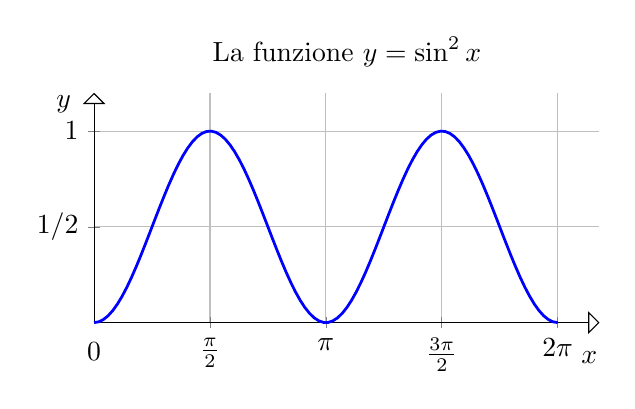
\begin{tikzpicture}
\begin{axis}[
   % etichette del grafico
     title={La funzione $y=\sin^2 x$},
     xtick={1.5708,3.1416,4.7124,6.2832},
     xticklabels={$\frac{\pi}{2}$,
                  $\pi$,$\frac{3\pi}{2}$,$2\pi$},
     ytick={0.5,1},yticklabels={$1/2$,$1$},
     grid=major,
   % dominio 2D
     domain=0:2*pi,
     xmin=0,xmax=6.85,
     ymin=0, ymax=1.2,
     samples=100,
   % assi
     axis x line=bottom,
     axis y line=left,
     every outer x axis line/.append style=
        {-open triangle 90},
     every outer y axis line/.append style=
        {-open triangle 90},
   % dimensioni tela
     width=8cm, height=4.5cm,
     clip=false
]
\addplot[color=blue, line width=1pt] {sin(deg(x))^2};
\node at (axis description cs:0,-0.125) {$0$};
\node at (axis description cs:0.98,-0.15) {$x$};
\node at (axis description cs:-0.06,0.95) {$y$};
\end{axis}
\end{tikzpicture}
\end{document}

